% !TEX TS-program = pdflatex
% !TEX encoding = UTF-8 Unicode

% This is a simple template for a LaTeX document using the "article" class.
% See "book", "report", "letter" for other types of document.

\documentclass[11pt]{article} % use larger type; default would be 10pt

\usepackage[utf8]{inputenc} % set input encoding (not needed with XeLaTeX)

%%% PAGE DIMENSIONS
\usepackage{geometry} % to change the page dimensions
\geometry{a4paper} % or letterpaper (US) or a5paper or....
% \geometry{margin=2in} % for example, change the margins to 2 inches all round
% \geometry{landscape} % set up the page for landscape
%   read geometry.pdf for detailed page layout information

\usepackage{graphicx} % support the \includegraphics command and options

% \usepackage[parfill]{parskip} % Activate to begin paragraphs with an empty line rather than an indent

%%% PACKAGES
\usepackage{booktabs} % for much better looking tables
\usepackage{array} % for better arrays (eg matrices) in maths
\usepackage{paralist} % very flexible & customisable lists (eg. enumerate/itemize, etc.)
\usepackage{verbatim} % adds environment for commenting out blocks of text & for better verbatim
\usepackage{subfig} % make it possible to include more than one captioned figure/table in a single float
% These packages are all incorporated in the memoir class to one degree or another...

%%% HEADERS & FOOTERS
% \usepackage{fancyhdr} % This should be set AFTER setting up the page geometry
% \pagestyle{fancy} % options: empty , plain , fancy
% \renewcommand{\headrulewidth}{0pt} % customise the layout...
% \lhead{}\chead{}\rhead{}
% \lfoot{}\cfoot{\thepage}\rfoot{}

%%% SECTION TITLE APPEARANCE
\usepackage{sectsty}
\allsectionsfont{\sffamily\mdseries\upshape} % (See the fntguide.pdf for font help)
% (This matches ConTeXt defaults)

%%% ToC (table of contents) APPEARANCE
\usepackage[nottoc,notlof,notlot]{tocbibind} % Put the bibliography in the ToC
\usepackage[titles,subfigure]{tocloft} % Alter the style of the Table of Contents
\renewcommand{\cftsecfont}{\rmfamily\mdseries\upshape}
\renewcommand{\cftsecpagefont}{\rmfamily\mdseries\upshape} % No bold!

% Package to insert code
\usepackage{xcolor}
\usepackage{listings}
\lstset{language=[ISO]C++}	%set code language
\lstset{basicstyle=\small\ttfamily,
		keywordstyle = \color{blue}\bfseries,
		commentstyle = \color{gray},
		stringstyle = \color{green}}	% code style
\lstset{tabsize=2}	% tabulation for code
\lstset{backgroundcolor = \color{yellow!7}}
\newcommand{\classname}[1]{\texttt{#1}}

% Maths packages
\usepackage{amssymb}
\usepackage{amsmath}

% Bellezza documento
\usepackage{microtype}

%%% END Article customizations

%%% The "real" document content comes below...

\title{BGLgeom library}
\author{Speranza Ilaria (matr. 854196) \\ Tantardini Mattia (matr. 858603)}
%\date{} % Activate to display a given date or no date (if empty),
         % otherwise the current date is printed 

\begin{document}
\maketitle
\newpage
\tableofcontents
\newpage

\section{Introduction}
	\subsection{Purpouse of the project}	%magari anche no??
	The purpose of the project is to extend the Boost Graph Library (BGL) providing it more functionalities to handle graph with geometric properties, that the BGL currently does not support. This mainly means to provide a graph from BGL, that already implements all topological operations, a way to describe its vertices as points and its edges as curves in the space (2 or 3 dimensional). Along with this, classes which implements these kind of geometrical properties must be able to carry out geometric and analytic operations, such as computation of first and second derivative of the edges and creation of numerical meshes on them. \newline
	All these geometric functionalities we developed are aimed at solving numerical problems which can be modelled using a graph, but which also are in a geometric setting or need it: for instance, to compute flows in a network of blood vessels, meshes are required to solve finite element problemst. \newline
	Along with this library we provide to example of specific application: one about intersection of fractures in fractured porous media, and one solving a simple diffusion problem on a vascular network. \newline
	A lot of other applications can take advantage from this library: vascular and neural network, electronic circuits, .... 


\section{The library}
	\subsection{Briefs on BGL}
	The BGL is a template library to create, handle and operate on graphs. It implements some different classes of graphs, all the topological operations concerning graphs, and a lot of graph algorithms.
	\newline\newline
	% Metto qui quello che ho messo nella documentazione? adjacency_list e tutto il resto? forse comunque ho bisogno di dire dell'adjacency list, ma
	Among all these functionalities, we decide to concentrate on a single class to describe a graph and on how implement in an easy to use way the geometrical properties. To explain in more details our implementation choices, we need to spend some words on how that class and the graph properties work.
	
		\subsubsection{The adjacency\_list class}
		\classname{adjacency\_list} is a template class which represents a graph with a two dimensional structure: 
		a \texttt{VertexList} and a \texttt{OutEdgeList} container. The first one stores all the vertices of the graph, and each vertex contains the other one-dimensional structure which is the list of all the out-edges leaving that vertex (so only out-edges if the graph is directed, all the edges if the graph is undirected). \newline
		The class has five template parameters and the full protoytpe is: \classname{adjacency\_list< OutEdgeList, VertexList, Directed, VertexProperties, EdgeProperties >}. \newline
		The first two template parameters allow to choose the types of the underlying containers for the bidimensional structure. Choosing them affects space complexity of the graph and efficiency of some operations, such as inserting and removing edges. In our work we always set them to the selector \classname{boost::vecS} (that stands for \texttt{std::vector}) for ease of use and since, form BGL documentation, it is in average the most performant choice for every topological operation. \newline
		The third template parameter obviously allows to choose between a directed or undirected graph.\newline
		The last two template parameters are the most interesting ones: they allow to choose what are the vertex and the edge properties. The BGL provides an easy way to handle them: the so called \textit{bundled properties}. They simply are classes, or better, structs, which can be passed as template parameter to the \classname{adjacency\_list} class, and they will become its vertex and edge properties, along with all their attributes and memeber functions. This gives a lot of flexibility: for instance, if we want all the vertices to have as properties three doubles, an int, two strings and a member that returns a random number, we only have to define them all in the same struct and pass it as the fourth template parameter of the \classname{adjacency\_list} class. The same for the edges, passing the corresponding struct as fifth template parameter. Moreover, the usage of a struct, instead of a class, enables public member access, and this comes out in a slight more ease of use when accessing the properties. \newline
		Concluding this description, we underline that choosing different values for the template parameters consits in changing the type of the graph one is using, with consequence on some other tool provided by BGL.
		
		\subsubsection{Vertex and edge descriptors}
		Two specific handles are provided to manipulate vertices and edges: the vertex and the edge descriptors. They may be of different types, depending on the graph type. They in general 'refer' to a particular vertex or edge, thus allowing for instance to access their properties, or to specify in a very readable way topological operations. \newline
		Two more tools are provided to access a graph: vertex and edge iterators. As the descriptors, the iterators can be of different types depending on the graph type. Specific function return the iterator to the first and last vertex and to the first and last edge in the graph, thus allowing graph traversal. Dereferencing an iterator one will obtain the descriptor of the vertex or edge pointed by that iterator. \newline
		Both descriptors and iterators are accessible through the \classname{graph\_traits} class.
		
		\subsubsection{Accessing properties}
		Using \textit{bundled properties}, BGL provides an easy way to acces vertex or edge properties: just use the \texttt{operator[]} on a graph object, with index the descriptor of the vertex or edge whose properties one wants; this will consists in accessing the struct used as vertex or edge property. Since a struct has public access, with the dot operator we can immediately read from or write in each attribute or call a member function.
		
		% Mettere del codice di esempio qui????
	
	
	\subsection{BGLgeom}
	This is the library we developed to meet the goals of the project. The name is the union of "BGL", since this wants to be an extension of it, and of "geom", that stands for "geometry", to indicate the aim of the main functionalities added. 
	\newline\newline
	The library comes from the need to have a common environment where to build and run very different types of applications, but with a geometrical setting and an underlying graph structure in common. This implies, besides the development of the geometric properties, the implementation of input/output utilities, to make this library produce useful outputs for other softwares. From this point of view, this library can be a common starting point for different projects and applications.
	\newline\newline	
	%We build a template library capable to handle 2 and 3 dimensional geometries. Most geometric characteristics, such as points, geometries for the edges, etc, are templatized on the dimension of the space. Another recurrent template parameter is the type of the graph used, needed in most cases to use the tools from BGL. 
	
		\subsubsection{What is inside}
		The library contains many things:
		\begin{itemize}
			\item \textbf{Adapters for BGL}: we provide some layers and additional functions to hidden the most used native BGL ones and to improve readibility and ease of use.
			\item \textbf{Classes to build graph properties}: the main part of the library are all the classes we developed to create for the graph a vertex and an edge property which include the basic geometric requirments.
			\item \textbf{Geometrical and numerical utilieties}: we included in this library some code to compute integrals, generate meshes, compute intersections between linear edges.
			\item \textbf{I/O utilities}: we provide one reader class to read tabular ASCII files, and three writer classes to produce three different types of output: ASCII, .pts and .vtp files.
			\item \textbf{Tests}: we provide source code examples to show how the main classes and writers work.
		\end{itemize}
	
		%forse posso dire prima quali proprietà geometriche abbiamo implemenmtato, come e perché, e poi come le abbiamo messe insieme per poter usare i grafi.
	
		\subsubsection{Geometric properties}
		In this library we do not provide any type of grap. We decided to use the \classname{adjacency\_list} class directly from the BGL, since this already gives a lot of flexibility. We focused on implementing the geometrical properties we was required as \textit{bundled properties} (that are really flexible too), so that we could simply pass them as template parameters to create a graph with the desired characteristics. Moreover, we chose to put in our properties only the functionalities that are really needed for a geometrical description, leaving the user the freedom to add its own characteristics and functionalities. \newline
		The geometric properties we were asked to developed are:
		\begin{itemize}
			\item Coordinates for points.
			\item Boundary conditions.
			\item Parameterization for the edges, along with computation of the main characteristics: first and second derivative, curvature, curvilinear abscissa.
			\item Meshes on the edges.
		\end{itemize}
		We templatized all this elements on the dimension of the space.				
		\paragraph{Points.}	To represent points we used \texttt{Eigen} matrices, with 1 column and n rows. We choose the \texttt{Eigen} because it provides high efficiency and a lot of numerical method to compute in an easy way geometrical quantities.
		\paragraph{Boundary conditions.} We implemented a class to store a boundary condition as a type and a value. We provide an \texttt{enum class BC\_type} to represent the most common types of boundary conditions.
		\paragraph{Edge geometries.} Concerning the geometry and parameterization of the edges, we were asked to be as generic as possible, that is the library would have been able to manage any possible parameterization of the type
		\begin{equation*}
			f:\mathbb{R}\rightarrow\mathbb{R}^{n} \quad, \quad n=2,3 ,
		\end{equation*}
		i.e. from a line to a generic curve in the plane or in the space. We met this goal by developing three different classes: the \classname{linear\_geometry} class for the straight lines, and the \classname{generic\_geometry} and \classname{bspline\_geometry} classes for a generic curve.\newline
		All this classes hold a parameterization of the curve inbetween 0 and 1, so we actually have parameterizations of the type
		\begin{equation*}
			f:[0,1]\rightarrow\mathbb{R}^{n} \quad, \quad n=2,3.
		\end{equation*}
		for each geometry. All classes derive from an abstract class, \classname{edge\_geometry}, which specifies the functionalities that the geometry of an edge should have: in our case, they are the evaluation of the curve, the computation of first and second derivative, curvature and curvilinear abscissa at given value (or a vector of values) of the parameter.
		%Descrizione di ogni geometry?
		\paragraph{Meshes.} We provide a class that is at the same time a mesh generator and a container for two type of meshes: the parametric one, generated from the parameterization of the edge, and the real one, that is the evaluation of the parametric mesh on the same edge. We decided to keep also the parametric mesh since it may be useful to evaluate it to get also other quantities, such as curvature, in correspondence of the points of the real mesh.
		
		% Implementation details di ogni classe? Forse con un po' di considerazioni sull'efficienza ci sta
		
		
		\subsubsection{Building a geometric graph}		
		\paragraph{The geometric base properties.} We developed the structs \classname{Vertex\_base\_property} and \classname{Edge\_base\_property}, that are thought to be the base vertex and edge property for a graph which wants to have a geometric description. They are substantially two containers, which gather the previous described classes.
		In the \classname{Vertex\_base\_property} we included:
		\begin{itemize}
			\item The coordinates of the point in the space representing the vertex.
			\item A \texttt{std::array} to store the boundary conditions on that vertex. We templatized the array on the number of the boundary conditions the user wants, since it may happen for some applications that more than one FEM problem has to be solved on the graph, thus requiring more than one boundary condition for each vertex.
		\end{itemize}
		In the \classname{Edge\_base\_property} we included:
		\begin{itemize}
			\item One of the geometry class.
			\item Our mesh class.
		\end{itemize}
		The \classname{Edge\_base\_property} is template on the geometry of the edges we want.
		Both properties are also provided with two more attributes: an index and a label. These may be useful to give to vertices and edges a specific ordering and to keep track of and reconnaise particular parts of the graph.
		\paragraph{A first Example.} To create a geometric graph with the above properties, we now only have to declare an object of class \classname{adjacency\_list} with \classname{Vertex\_base\_property} as fourth template parameter and with \classname{Edge\_base\_property} as fifth template parameter. For instance:
\begin{lstlisting}[frame=single]
using Edge_prop = 
	BGLgeom::Edge_base_property< BGLgeom::linear_geometry<3>, 3 >;
using Vertex_prop = BGLgeom::Vertex_base_property<3>;
using Graph = 
	boost::adjacency_list< boost::vecS, boost::vecS, 
		boost::directedS, Vertex_prop, Edge_prop >;
Graph G;
\end{lstlisting}
		Note that the we created and empty graph and that all the properties, especially geometries for edges, have to be set up with all the needed values while building the graph. Moreover, note that, since the chosen geometry for the edge properties \texttt{Edge\_prop } is \texttt{linear\_geometry}, and since this \texttt{Edge\_prop} is passed as template argument to the \classname{adjacency\_list} class, the whole graph will have edges with linear geometry. This is a kind of 'static' property of the graph. A future development of the library may consider to create a kind of 'dynamic' \texttt{Edge\_base\_property}, that is capable to hanlde different geometries on different edges. %Maybe lo possiamo mettere nei todo's questo. 
		\paragraph{Extending base properties.} We created our first new geometric graph with the properties provided by our library. But in the applications a lot of other quantities and parameters may be necessary, for instance diameter and pressure for a blood vessel, or permeability for fractures, or any other kind of variable. How to expand the basic geometric properties of vertices and edges we provide to contain the new variables? Just publicly inherit from our base properties, and define at least a default constructor. This is not mandatory unless you use pointers in your derived properties, but we strongly suggest to implement it to prevent bad behaviours. A generic example is:
\begin{lstlisting}[frame=trbl]
struct My_vertex_prop : public BGLgeom::Vertex_base_property<3> {
	double variable1;			// may be pressure
	int varaible2;				// some flag
	std::string a_string;	// a description
	my_class object;			// may be solver for FEM problem on edge
	
	My_vertex_prop() : BGLgeom::Vertex_base_property<3>(),
										variable1(.0),
										variable2(0),
										a_string(),
										object() {};	
};
\end{lstlisting}
		The use of inheritance is a fast way to derive your own vertex or edge property with a lot of freedom, and also allows access in a fast and easy way to the inherited geometric properties.
		\paragraph{Adding vertices and edges.} To add new edges and vertices to a graph the user substanqially uses the already existent \texttt{boost} functions which make that job. We only hid them under external functions which recall the name: \texttt{BGLgeom::new\_vertex} and \texttt{BGLgeom::new\_edge} instead of \texttt{boost::add\_vertex} of \texttt{boost::add\_edge}. We provided different overloads: just adding vertex and edge, adding them along with their properties, performing additional checks on the insertion of the edges. Furthermore, we added three new functions (\texttt{BGLgeom::new\_linear\_edge}, \texttt{BGLgeom::new\_generic\_edge} and \texttt{BGLgeom::new\_bspline\_edge}) to add edges, to provide an easy way to add a new edge to the graph already with its geometry set up in the proper way.	On how to use the functionality we provided to build a graph, see the source code \textit{test\_BGL\_vs\_BGLgeom.cpp}.
	
		\subsubsection{Reader class}
		We wanted to give a tool to read graph topology and properties directly from file. Since the properties are così che non le sappiamo, dobbiamo leggere every type of file, quindi bella lì ASCII! Scegliamo te.
		
		\subsubsection{Writer classes}

	
	
	
	% Mettere delle subsubsection con tipo le classi principali, cosa fanno, perché fatte così, ecc
	
	\subsection{Todos}	%???


\section{Applications}

	In this section we present two examples from real situations, where some tools of BGLgeom library prove to be useful.

	\subsection{Fracture Intersection}
	In this example a list of fractures, all lying on the same plane, is given as input. The goal is to build a graph representing the network, with vertices in correspondence of the fractures' extremities and of the intersection points  and edges representing the fractures. A very simple example is shown in figure \label{fig:frac_int}.
	\begin{figure}
		\centering 
		%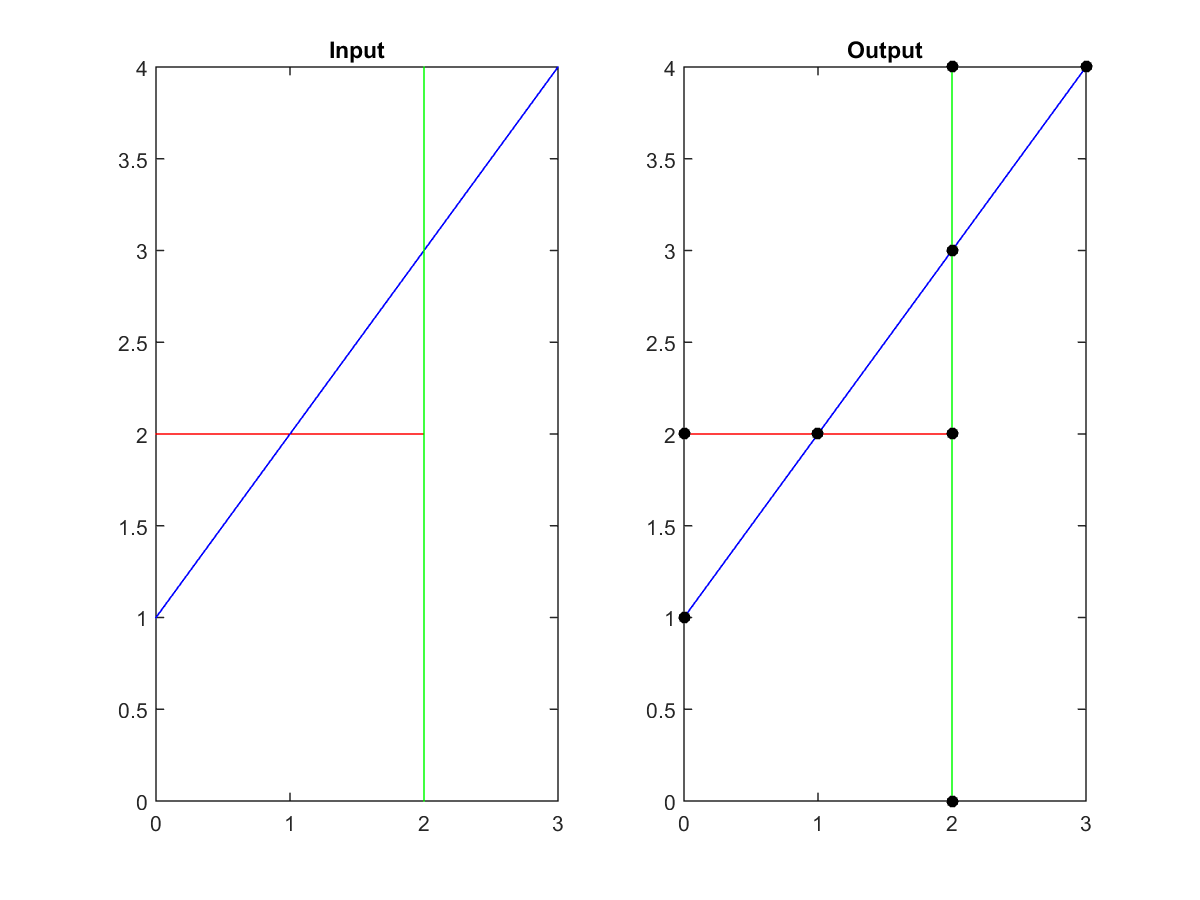
\includegraphics[width=0.5\textwidth]{frac_inters}
		\caption{Example}
		\label{fig:frac_int}
	\end{figure}
	
		\subsubsection{Intersection types}
		To compute the intersection between two given edges we use a piece of code, developed by Professor Formaggia, which we included as a utility in our libary BGLgeom, after adapting it to our specific data structeres: it outputs the number of intersections, the intersection point (if the intersection is not just a point but a segment, its two extremes are returned) and two boolean variables, whose value depends respectively on the parallelism and the collinearity of the evaluated edges. \newline
		We identified 11 different types of intersection between two linear edges (see figure ...): we built then a layer class which associates each possible outcome of Professor Formaggia's code with one and only one of the overmentioned 11 intersection types. \newline
			
		



	\subsection{Diffusion on vascular network}

	%Computational issues?? Complexity and time efficiency?

\end{document}
